%!TEX program = xelatex
\documentclass[11pt,utf8]{article}
    \usepackage[no-math,cm-default]{fontspec}
    \usepackage{amsmath}
    \usepackage{amsthm}
    \usepackage{amssymb}
    
    %\usepackage{xeCJK}
    \usepackage{verbatim}
    \usepackage{indentfirst}
    \usepackage{syntonly}
    \usepackage{fancyhdr}
    \usepackage[unicode=true, colorlinks, linkcolor=black, anchorcolor=black, citecolor=black, urlcolor=black]{hyperref}
    \usepackage{graphicx}
    \usepackage[top = 1.2in, bottom = 1.2in, left = 1.3in, right = 1.3in]{geometry}
    \usepackage{xcolor}
    \usepackage{paralist}
    \usepackage{ulem}
    \usepackage{titlesec}
    \usepackage{zhspacing}
    \usepackage{booktabs}
    \usepackage{multirow}
    \usepackage{multicol}
    \usepackage{supertabular}
    
    \defaultfontfeatures{Mapping=tex-text}
    \zhspacing
    %\setromanfont{Computer Modern Roman}
    \newfontfamily\zhfont[BoldFont=Adobe Heiti Std,ItalicFont=Adobe Kaiti Std]{Adobe Song Std}
    \setmonofont[Scale=1]{Courier New}
    \XeTeXlinebreaklocale "zh"
    \XeTeXlinebreakskip = 0pt plus 1pt
    
    \usepackage{diagbox}
    
    \begin{document}
    
    \let\enumerate\compactenum
    \let\endenumerate\endcompactenum
    \let\itemize\compactitem
    \let\enditemize\endcompactitem
    \setlength{\pltopsep}{5pt}
    \setlength{\parindent}{2em}
    \setlength{\footskip}{30pt}
    \setlength{\baselineskip}{1.3\baselineskip}
    \renewcommand\arraystretch{1.2}
    
    
    \title{人工神经网络\\第一次作业\\MNIST Digits Classification with CNN}
    \date{2017年10月25日}
    \author{计55 张卡尔 2015011025}
      \maketitle
      \section*{实验内容}
        \indent 本实验将会使用卷积神经网络实现MNIST手写数字识别分类,对不同的网络结构以及不同的参数进行讨论,与MLP进行对比,探索优化方法及策略。\\
      \section*{网络结构设计}
        本实验主要使用的网络结构如下:
        \begin{itemize}
          \item 输入层($N*28*28$)
          \item 卷基层($N*4*28*28$, 卷积核大小$3*3$)
          \item Relu层
          \item 池化层 ($N*4*14*14$)
          \item 卷基层($N*4*14*144$, 卷积核大小$3*3$)
          \item Relu层
          \item 池化层 ($N*4*7*7$)
          \item 全连接层($N*196*10$)
          \item Softmax交叉熵损失层
        \end{itemize}
        
        \section*{训练参数探究}
          
          \subsection*{损失函数函数}
            \indent 使用相同参数、相同结构的上述网络,分别使用Euclidean和SoftmaxCrossEntropy两种损失函数训练100个epoch,对比结果如下。\\
            
            \begin{table}[h]
              \centering
              \begin{tabular}{|c|c|c|c|c|c|c|}\hline
                策略&训练集loss&测试集loss&训练集acc&测试集acc&训练时间&参数个数\\\hline
                Euclidean&0.087&0.088&96.75\%&96.78\%&233分钟&2158\\
                SoftmaxCrossEntropy&0.046&0.043&98.56\%&98.65&233分钟&2158\%\\\hline
              \end{tabular}
              \caption{损失函数对比表}
              \label{tab:Margin_settings}
            \end{table}

            \begin{figure}
              \begin{center}
                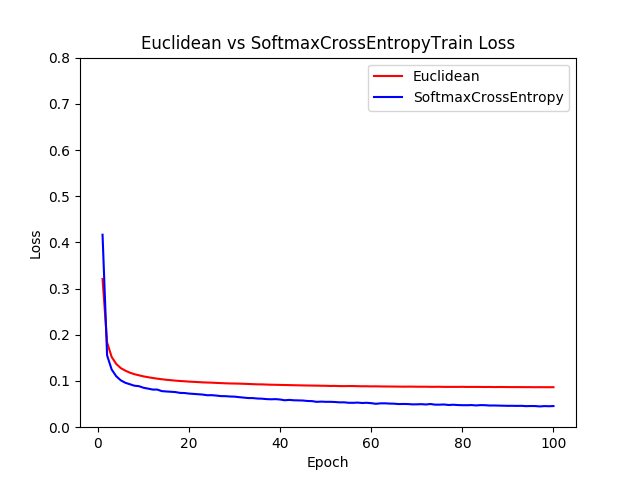
\includegraphics[width=7cm]{result/EuclideanvsSoftmaxCrossEntropy_loss.png}
                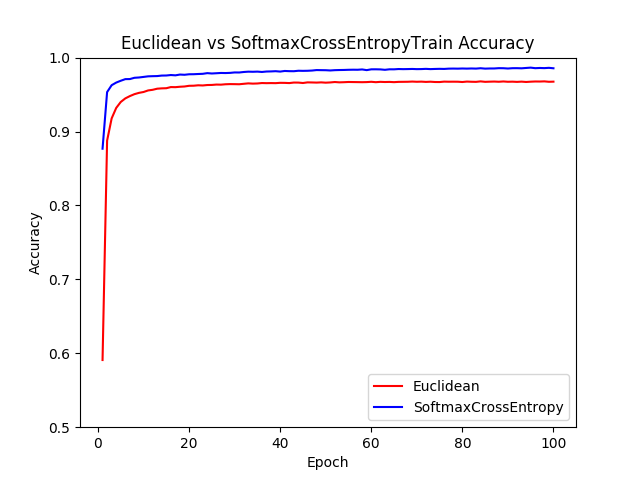
\includegraphics[width=7cm]{result/EuclideanvsSoftmaxCrossEntropy_acc.png}\\
                \caption{损失函数对比图}
              \end{center}
            \end{figure}
            
            \indent \indent 通过对比,可以发现在使用相同的参数和网络结构对同一任务进行训练时,在训练相同数量的epoch的情况下,Relu比Sigmoid收敛速度更快且最终精确度更高,损失值更小。分析其原因,我认为是Sigmoid函数本身的特点导致的。Sigmoid函数在中间部分的梯度较高,在两侧梯度很低,导致训练到一定程度时,梯度越来越小,从而训练速度十分缓慢。而Relu函数在$[0, \infty) $上的梯度为常数,不会出现梯度消失的问题,因而收敛速度更快,且能够在更少数量的epoch上达到比较高水平的精准度。\\
            \indent 在训练时间方面,Sigmoid网络花费了$51'53''$,Relu网络花费了$57'26''$,相差不大。
          \subsection*{Learning Rate}
            
          \subsection*{初始权重}
            \begin{table}[h]
              \centering
              \begin{tabular}{|c|c|c|c|c|c|c|}\hline
                策略&训练集loss&测试集loss&训练集acc&测试集acc&训练时间&参数个数\\\hline
                init\_std=0.1&0.045&0.047&98.66\%&98.52\%&233分钟&2158\\
                init\_std=1&0.046&0.043&98.56\%&98.65\%&233分钟&2158\\\hline
              \end{tabular}
              \caption{初始权重对比}
              \label{tab:Margin_settings}
            \end{table}
            \begin{figure}
              \begin{center}
                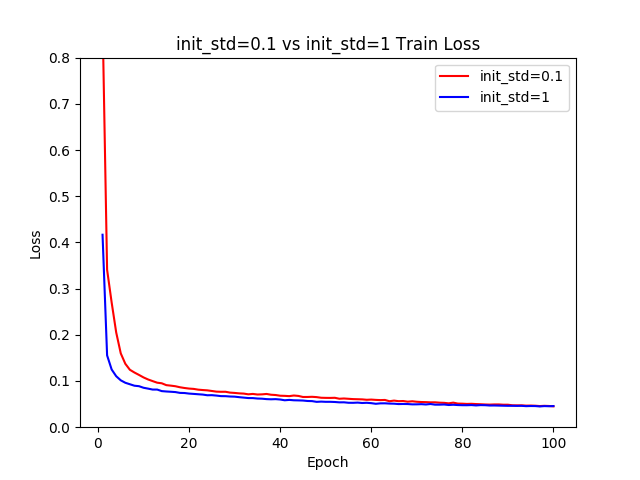
\includegraphics[width=7cm]{result/init_std=0.1vsinit_std=1_loss.png}
                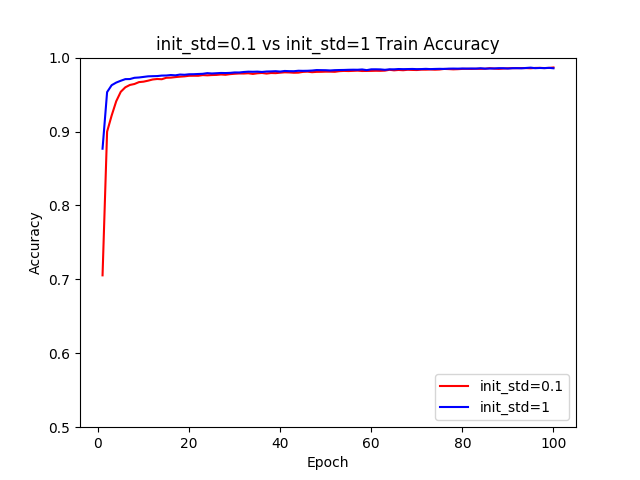
\includegraphics[width=7cm]{result/init_std=0.1vsinit_std=1_acc.png}\\
                \caption{初始权重对比图}
              \end{center}
            \end{figure}
          

          \subsection*{通道数}
            \begin{table}[h]
              \centering
              \begin{tabular}{|c|c|c|c|c|c|c|}\hline
                策略&训练集loss&测试集loss&训练集acc&测试集acc&训练时间&参数个数\\\hline
                8通道&0.029&0.028&99.08\%&99.10\%&540分钟&4584\\
                4通道&0.046&0.043&98.56\%&98.65\%&233分钟&2158\\\hline
              \end{tabular}
              \caption{通道数对比表}
              \label{tab:Margin_settings}
            \end{table}
            \begin{figure}
              \begin{center}
                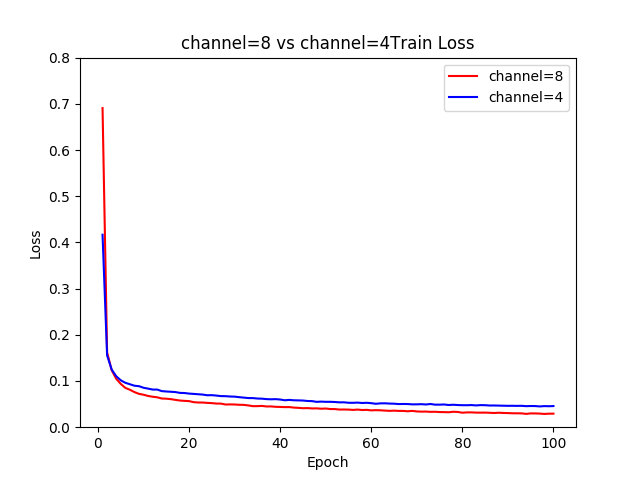
\includegraphics[width=7cm]{result/channel=8vschannel=4_loss.png}
                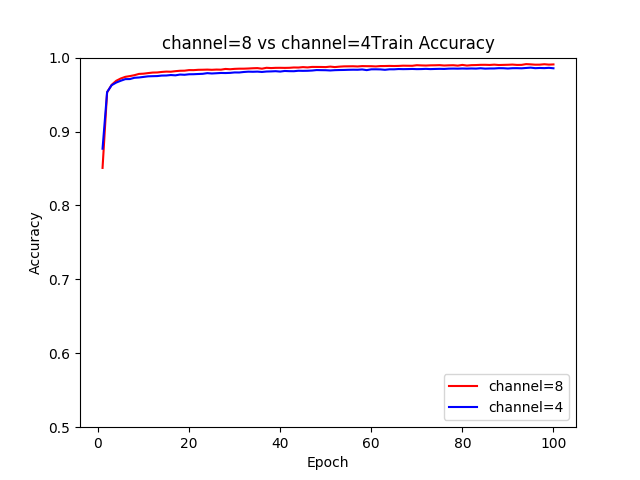
\includegraphics[width=7cm]{result/channel=8vschannel=4_acc.png}\\
                \caption{通道数对比图}
              \end{center}
            \end{figure}
          \subsection*{其他参数}
            \indent 由于本次实验时间有限,之前几个参数的调整过程占用时间过长,其他参数的优化问题在本次实验中没有深入研究。batch\_size使用的是常规的100,weight\_decay由于在其他参数尚未优化之前效果不明显,故暂取为0。\\
        \section*{实验总结}
          \indent 本次实验占用了我很多的时间,收获也是十分丰富的。我走了许多弯路,例如在一开始在寻找正常的高准确度上浪费了许多时间,由于有多个参数未调,因此有时候会同时修改了多个参数,导致找到了一个相对较优的参数就开始进行优化算法的实现。但其实后来才发现把learning rate调大以后甚至比现在做过优化的算法效果还好。总而言之,通过这次实验我真实体会到了网络结构、激励函数、参数这些对网络效果的影响。只有真正理解了每一个数值的具体含义和其对网络的影响,才能进行合理的调参。\\
      
    \end{document}